% Autor: Leonhard Segger, Alexander Neuwirth
% Datum: 2017-10-30
\documentclass[
	% Papierformat
	a4paper,
	% Schriftgröße (beliebige Größen mit „fontsize=Xpt“)
	12pt,
	% Schreibt die Papiergröße korrekt ins Ausgabedokument
	pagesize,
	% Sprache für z.B. Babel
	ngerman
]{scrartcl}

% Achtung: Die Reihenfolge der Pakete kann (leider) wichtig sein!
% Insbesondere sollten (so wie hier) babel, fontenc und inputenc (in dieser
% Reihenfolge) als Erstes und hyperref und cleveref (Reihenfolge auch hier
% beachten) als Letztes geladen werden!

% Silbentrennung etc.; Sprache wird durch Option bei \documentclass festgelegt
\usepackage{babel}
% Verwendung der Zeichentabelle T1 (Sonderzeichen etc.)
\usepackage[T1]{fontenc}
% Legt die Zeichenkodierung der Eingabedatei fest, z.B. UTF-8
\usepackage[utf8]{inputenc}
% Schriftart
\usepackage{lmodern}
% Zusätzliche Sonderzeichen
\usepackage{textcomp}

% Mathepaket (intlimits: Grenzen über/unter Integralzeichen)
\usepackage[intlimits]{amsmath}
% Ermöglicht die Nutzung von \SI{Zahl}{Einheit} u.a.
\usepackage{siunitx}
% Zum flexiblen Einbinden von Grafiken (\includegraphics)
\usepackage{graphicx}
% Abbildungen im Fließtext
\usepackage{wrapfig}
% Abbildungen nebeneinander (subfigure, subtable)
\usepackage{subcaption}
% Funktionen für Anführungszeichen
\usepackage{csquotes}
% Zitieren, Bibliographie
\usepackage{biblatex}


% Zur Darstellung von Webadressen
\usepackage{url}
%chemische Formeln
\usepackage[version=4]{mhchem}
% siunitx: Deutsche Ausgabe, Messfehler getrennt mit ± ausgeben
\usepackage{floatrow}
\floatsetup[table]{capposition=top}
% Verlinkt Textstellen im PDF-Dokument
\usepackage[unicode]{hyperref}
% "Schlaue" Referenzen (nach hyperref laden!)
\usepackage{cleveref}
\sisetup{
	locale=DE,
	separate-uncertainty
}
%\bibliography{6Mi_M3_29-11-2017_References}

\begin{document}
	
	\begin{titlepage}
		\centering
		{\scshape\LARGE Versuchsbericht zu \par}
		\vspace{1cm}
		{\scshape\huge M5 - Jo-Jo und Kreisel\par}
		\vspace{2.5cm}
		{\LARGE Gruppe 6Mi \par}
		\vspace{0.5cm}
		
		{\large Alexander Neuwirth (E-Mail: a\_neuw01@wwu.de) \par}
		{\large Leonhard Segger (E-Mail: l\_segg03@uni-muenster.de) \par}
		\vfill
		
		durchgeführt am 13.12.2017\par
		betreut von\par
		{\large Kristina Mühlenstrodt} %TODO Anpassen
		
		\vfill
		
		{\large \today\par}
	\end{titlepage}
	\tableofcontents
	\newpage

	%TODO mehr TODO in Default	

	\section{Kurzfassung}
	Um das Prinzip von Jo-Jos und Kreiseln zu untersuchen wurden zwei Experimente durchgeführt.
	Das Erste untersucht das Maxwell'sche Fallrad.
	Dabei wurde einmal mithilfe des Trägheitsmoments und einmal durch Messung der Falldauer in Abhängigkeit von der Fallhöhe der Abrollradius bestimmt und die beiden Ergebnisse verglichen.
	Dabei war zu erwarten, dass die Unsicherheiten der beiden Ergebnisss überschneiden.
	%TODO Abrollradius Ergebnis
	\par
	Im zweiten Versuch wurde die Präzession eines schweren, symmetrischen Kreisels untersucht. 
	Daraus wurde das Trägheitsmoment bestimmt und mit dem Trägheitsmoment, das aus Masse und Abmessungen bestimmt wurde, verglichen.%Trägheitsmoment des Kreisels?
	Auch hier war zu erwarten, dass die Werte innerhalb der Vertrauensbereiche übereinstimmen.
	%TODO Trägheitsmoment Ergebnis
	\section{Methoden}
	%TODO Bilder von der Website klauen
	\subsection{Maxwell'sches Fallrad}
	Zunächst wurde die Fallzeit eines Maxwell'schen Fallrads in Abhängigkeit vom Fallweg für fünf verschiedene Fallhöhen je fünf mal gemessen.
	\begin{figure}[tb]
		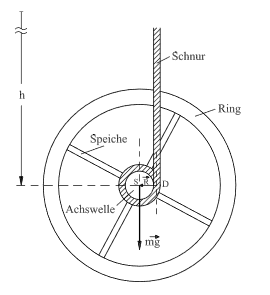
\includegraphics[width=0.4\textwidth]{Fallrad}
		\centering
		\caption{Maxwell'sches Fallrad}
		\label{Fallrad}
		\centering
	\end{figure}
	Der Aufbau eines Maxwell'schen Fallrads ist in \cref{Fallrad} dargestellt \footnote{Jo-Jo und Kreisel Einführung, Zugriff am 18.12.2017}.
	Dann wurde das Rad gewogen und mit einer Schieblehre ausgemessen, um daraus das Trägheitsmoment bestimmen zu können.
	Dabei wurde Dicke, Außenradius und Innenradius sowie die Dicke des Aufhängefadens an fünf verschiedenen Stellen gemessen, um dann über diese Werte mitteln zu können, da diese Werte besonders bedeutend für das Trägheitsmoment bzw. den Abrollradius sind.
	
	\subsection{Kreisel}
	Dann wurde ein schwerer, symmetrischer Kreisel untersucht.
	Dieser hatte die Form einer Metallkugel, in der in radialer Richtung eine Stange eingeschraubt war, auf der sich eine verschiebbare Zusatzmasse befand.
	Um die eine möglichst reibungsfreie Bewegung des Kreisels und die Eigenschaft der Schwere zu ermöglichen, war dabei die Kugel auf einem durch Pressluft in einer Hohlhalbkugel erzeugten Luftpolster gelagert.
	Die Eigenfrequenz der Kugel wurde dabei mit einem Pressluftstrahl aus einer Düse manuell kontrolliert.
	Zunächst wurde die Kugel gewiegt und ihr Durchmesser mit einer Schieblehre bestimmt.
	Dann wurde bei waagerechter Achse die Kraft bestimmt, mit der das Gewicht der Achse und des Zusatzgewichtes im Abstand $ l $ die Achse nach unten zieht, um die Größe $ amg$ bestimmen zu können.%bissl unschön
	Diese Messung wurde für drei Abstände der Zusatzmasse von der Kugel je fünf mal durchgeführt.
	Nachdem die Kugel mit dem Pressluftstrahl beschleunigt wurde, wurde die Eigenfrequenz mit einem Stroboskop mit verstellbarer Frequenz bestimmt.
	Dazu wurde die Frequenz des Stroboskop solange verringert, bis der Kreisel im Licht der Stroboskoplampe scheinbar stillsteht und die Markierung auf der Kugel nur einmal sichtbar ist.
	Sobald dies erfüllt war wurde die Frequenz vom Stroboskop abgelesen und mit der Pressluftdüse versucht diese möglichst konstant zu halten, was dadurch erkennbar war, ob die Markierung auf der Kugel sich scheinbar bewegte.
	Dann wurde mit einer Stoppuhr die Präzessionszeit der Kreiselachse bestimmt.
	Dabei wurde nur eine Umdrehung gemessen, um die Abweichung der Eigenfrequenz gering halten zu können.
	Diese Messung wurde für dieselben drei Abstände der Zusatzmasse von der Kugel wie zuvor durchgeführt.
	
	
	\section{Ergebnisse und Diskussion}
	%TODO Datenanalyse -> Überschrift?
	%TODO Unsicherheiten
	

	\subsection{Beobachtung}
	\subsubsection{Fallrad}
	\subsubsection*{Fallzeitbetrachtung}%TODO Titel
	In den Graphen \cref{HoeheGegenZeit} und \cref{HoeheGegenZeitquadrat} sind die Fallhöhen gegen die Fallzeiten, bzw deren Quadrate, aufgetragen.
	\cref{BeschleunigungGegenZeit} zeigt das Verhältnis der Fallhöhen zu den Fallzeitquadraten in Abhängigkeit von der Fallzeit.
	Der lineare Zusammenhang ist beim Betrachten der Werte bereits erkennbar und außerdem sollte dieser auch der Theorie zufolge auftreten (\cref{FallGleichung}).
	\begin{equation}
		h(t) = \frac{1}{2} g \frac{mR^2}{mR^2+J_S} t^2 = \frac{1}{2} g^* t^2
		\label{FallGleichung}
	\end{equation}
	Deshalb haben wir einen Fit mit dem \enquote{Scaled Levenberg-Marquardt}-Algorithmus, welcher die Methode der kleinsten Quadrate verwendet, durchgeführt.
	Für den Fit wurde die folgende Funktion zugrunde gelegt:
	\begin{equation}
		f(x)=A*x+B
	\end{equation}
	Es ergibt sich ein y-Achsenabschnitt von \SI{0,01754\pm 0,00049}{m/s^2}, welcher $\frac{1}{2}g^*$ entspricht. Der Fit weißt zwar eine minimale Steigung auf, diese ist jedoch vernachlässigbar, da sie im Verhältnis zur Unsicherheit des y-Achsenabschnitts auf dem Messintervall verschwindet. Folglich ergibt sich ein $g^*$ von \SI{0,03508 \pm 0,00098}{m/s^2}.
	\begin{figure}[tb]
		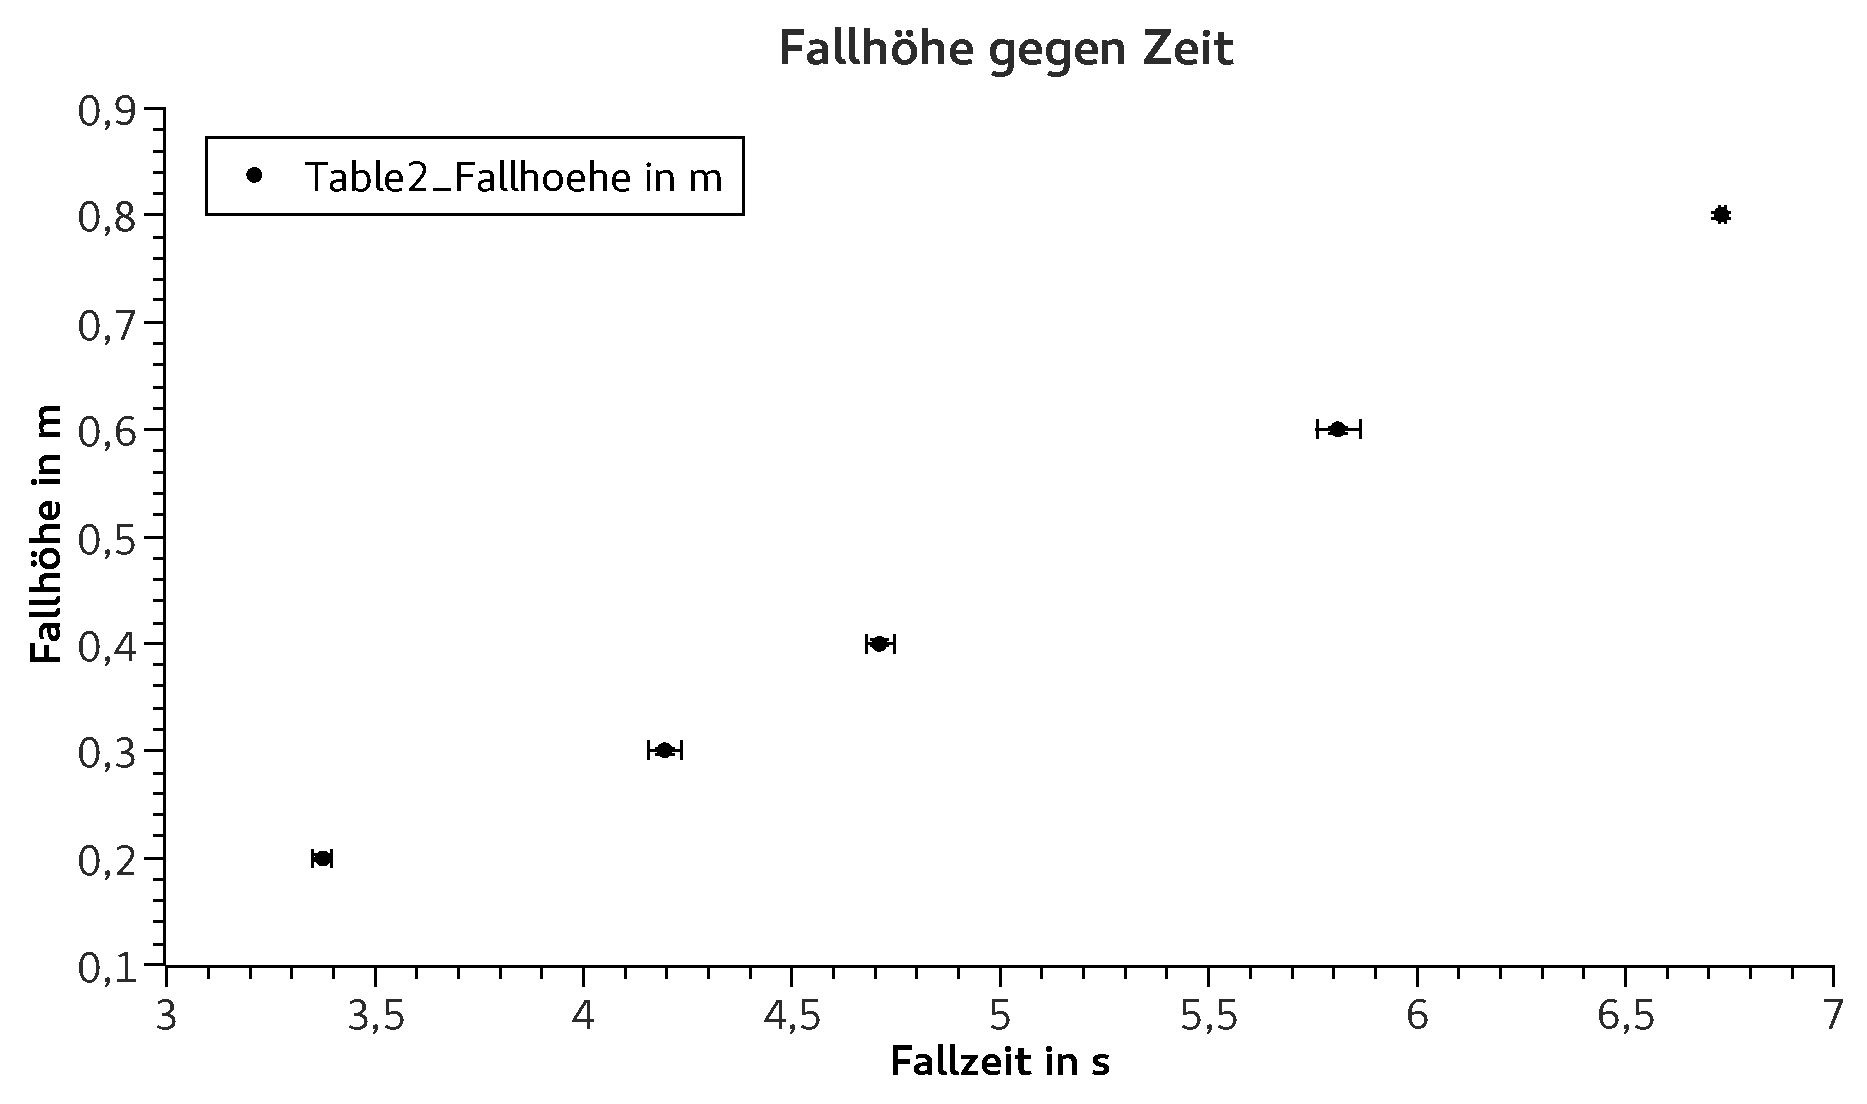
\includegraphics[width=1\textwidth]{HoeheGegenZeit}
		\centering
		\caption{Die Fallhöhe des Fallrads ist gegen die Fallzeit aufgetragen.}
		\label{HoeheGegenZeit}
		\centering
	\end{figure}
	\begin{figure}[tb]
		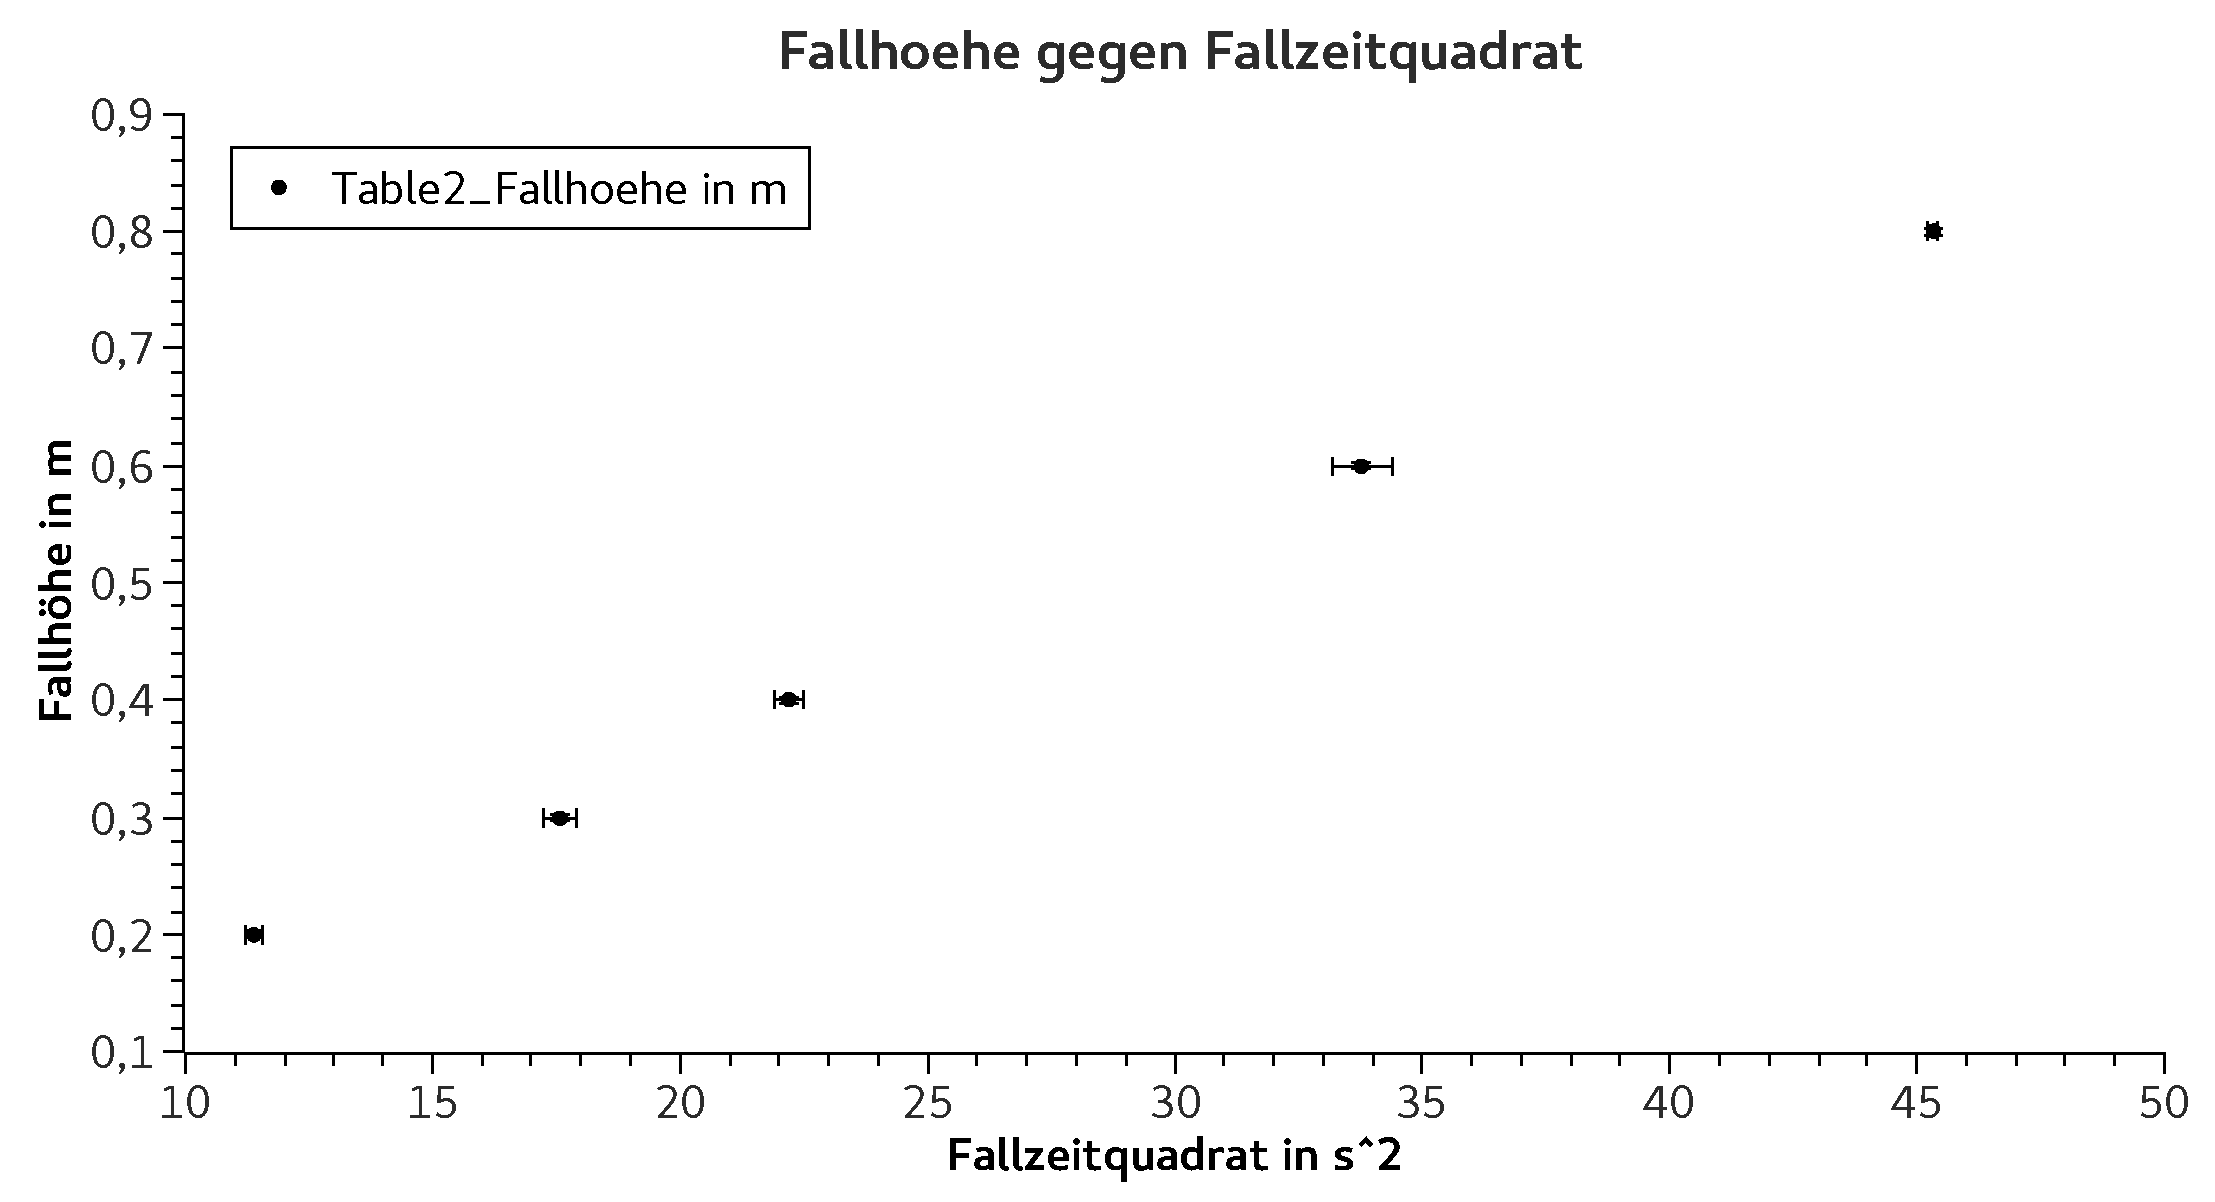
\includegraphics[width=1\textwidth]{HoeheGegenZeitquadrat} %TODO Graphen Skalierungen und Titel
		\centering
		\caption{Die Fallhöhe des Fallrads ist gegen die Fallzeitquadrate aufgetragen.}
		\label{HoeheGegenZeitquadrat}
		\centering
	\end{figure}
	\begin{figure}[tb]
		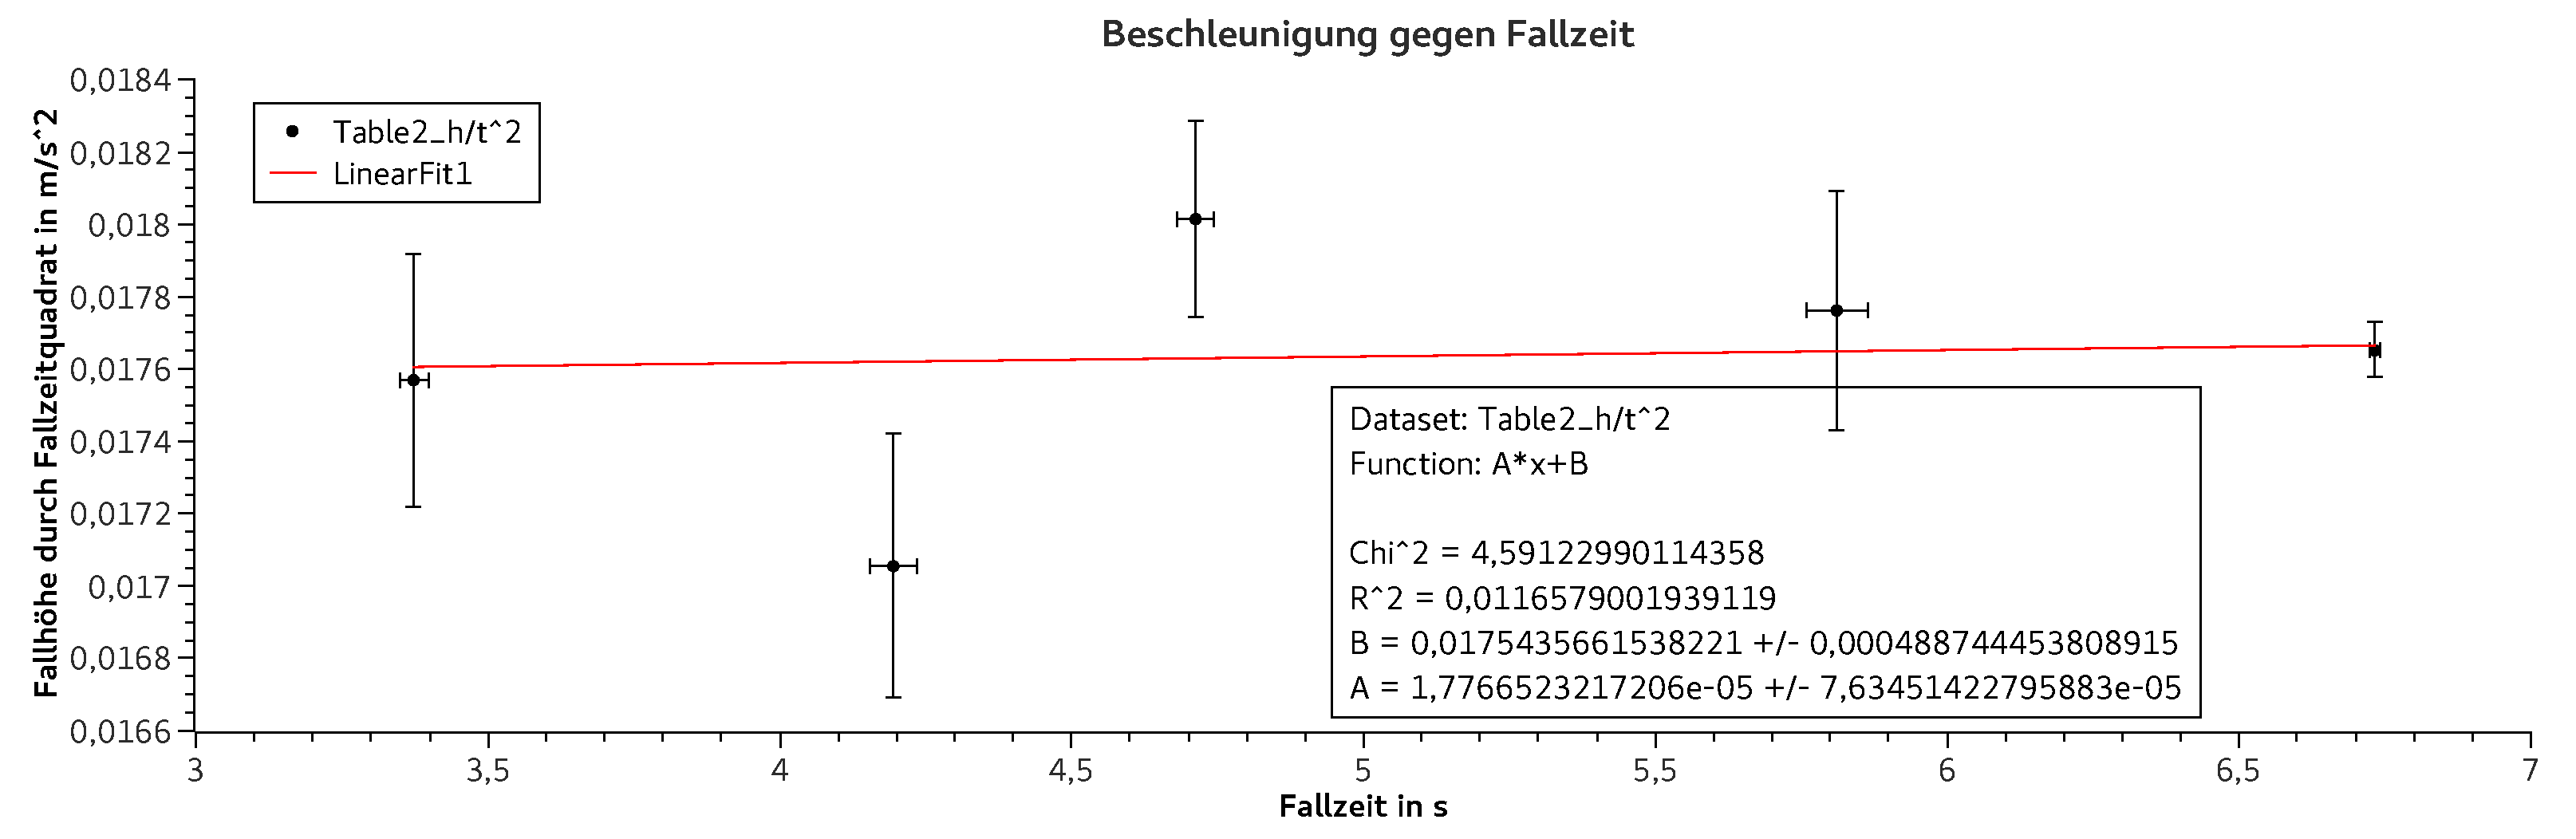
\includegraphics[width=1\textwidth]{BeschleunigungGegenZeit} %TODO ist nicht bescheunigung sondern 0.5Beschleunigung
		\centering
		\caption{Die halbe Beschleunigung des Fallrads ist gegen die Fallzeit aufgetragen.}
		\label{BeschleunigungGegenZeit}
		\centering
	\end{figure}



	\subsubsection*{Berechnung des Trägheitsmoments}
	Das Trägheitsmoments des Fallrads setzt sich aus den Trägheitsmomenten der einzelnen Komponenten zusammen.  %TODO Fallrads oder rades,... Duden sagt beides
	In \cref{Tabelle_Traegheitsmomente_Zylinder} sind Volumen und Trägheitsmoment von Zylindern aufgeführt. 
	Die Masse $m$ ergibt sich jeweils aus 
	\begin{equation}
		m = M \frac{V}{V_\text{ges}} 
	\end{equation}
	wobei $M$ die Masse des gesamten Fallrads und $V_\text{ges}$ entsprechend das gesamte Volumen ist. Es wird davon ausgegangen, dass der Stoff homogen ist. % => Dichte konstant + gleiche Zusammensetzung

	\begin{table}[tb]
		\centering
		\begin{tabular}{ r |  c | c | c}
			Zylinder& Volumen V &Rotationsachse & Trägheitsmoment $J$\\ \hline
			Vollzylinder& $\pi lr^2$ &Symmetrieachse & $\frac{1}{2} m r^2$ \\
			Vollzylinder& $\pi lr^2$&Querachse & $\frac{1}{4} m r^2 + \frac{1}{12} m l^2$ \\
			Hohlzylinder& $\pi l(r_2^2 - r_1^2)$&Symmetrieachse & $\frac{1}{2} m (r_1^2 + r_2^2)$ \\
		\end{tabular}
		\caption{Trägheitsmomente von (Hohl-)Zylindern zu verschiedenen Achsen.}
		\label{Tabelle_Traegheitsmomente_Zylinder} 
	\end{table}

	\begin{table}[tb]
		\centering
		\begin{tabular}{ r |  c | c }
			& Länge $L$ & Radius $R$\\ \hline
			Speiche &\SI{15,576\pm 0,023}{cm} & \SI{0,407\pm0,006}{cm}\\
			Achse & \SI{20,21\pm0,012}{cm} & \SI{0,405\pm0,006}{cm}\\
			Rad außen&- & \SI{9,007\pm0,001}{cm} \\
			Rad innen&- & \SI{7,788\pm0,012}{cm} \\
			Dicke Rad & \SI{1,15\pm0,004}{cm} & -
		\end{tabular}
		\caption{ Gemessene Längen.}
		\label{Tabelle_Laenge} 
	\end{table}
	Es folgt das Trägheitsmoment mit einer Gesamtmasse $M$ von \SI{0,76807 \pm 0,000028}{kg}:
	\begin{equation}
		J = \frac{1}{2}\frac{M}{2V_S+V_A+V_R} ( V_A R_A^2 + V_S (R_S^2 + \frac{1}{3} L_S^2) + V_R (R_\text{Rad,Außen}^2 + R_\text{Rad,Innen}^2)
	\end{equation}

	\begin{equation}
		u(y) = \sqrt{  \sum_{i=0}^{N} \left( \frac{\partial f}{\partial x_i}u(x_i)\right)^2  }
		\label{Partielle_Unsicherheiten}
	\end{equation}
	Beim Einsetzten aller Größen ergibt sich ein Trägheitsmoment von $J = \SI{42.550 \pm 0,1875}{kg cm^2}$ mit einer relativen Abweichung von 0,441\%. %TODO Texte Über Unsicherheiten bzw. Anhang
	\subsubsection*{Bestimmung des Abrollradius}
	Aus
	\begin{align}
		g^* &= \frac{gMR^2}{MR^2+J_S} \\
		\Rightarrow R^2 &= \frac{J_Sg^*}{gM-g^*M}
	\end{align}
	folgt, dass der Abrollradius durch 
	\begin{equation}
		R = \sqrt{\frac{J_S}{M}\frac{g^*}{g-g^*}}
	\end{equation}
	berechnet werden kann. 
	Setzt man die zuvor ermittelten Werte von $g^*$, $J_S$ und $M$ ein erhält man einen Abrollradius von \SI{0,446 \pm 0,006}{cm} mit einer Unsicherheit von ca. 1,5\%. 
	Der Radius der Achse beträgt \SI{0,405 \pm 0,006}{cm} und der Radius des Fadens \SI{0,052\pm 0,002}{cm}. 
	Folglich ergibt sich ein Abrollradius von \SI{0,457 \pm 0,006}{cm}.

	\subsubsection{Kreisel}
	\subsubsection*{Bestimmen des Trägheitsmomets}
	Für eine homogene Kugel gilt für das Trägheitsmoment, falls die Achse durch den Mittelpunkt läuft:
	\begin{equation}
		\label{KugelTraegheitsmoment}
		J_2=\frac{2}{5}m_kr_k^2
	\end{equation}
	Es folgt eine Trägheitsmoment für den gesamten Kreisel mit den gemessenen Größen $m_k = \SI{512,16\pm 0,028}{g}$ und $r_k = \SI{2,54\pm 0,006}{cm}$ von:
	\begin{equation}
		J = J_1 + J_2 = \SI{15}{g cm^2} + \SI{1321,70\pm 6,24}{g cm^2} = \SI{1336,70 \pm 6,24}{g cm^2}
	\end{equation}


	\subsection{Diskussion}
	%TODO Bezug/Nutzten oder sonst was
	
	\section{Schlussfolgerung}
	%TODO Rückgriff auf Hypothese
	
	%TODO Quellen zitieren, Websiten mit Zugriffsdatum
	%TODO Verweise auf das Laborbuch (sind erlaubt)
	%TODO Tabelle + Bilder mit Beschriftung
	\section{Beantwortung der Aufgaben zur Vorbereitung}
	\begin{enumerate}
		\item 
			\begin{align}
				0 = \frac{dE}{dt} &= \frac{d}{dt}(\frac{1}{2} m v^2 + \frac{1}{2} J_S \omega^2 - mgh) \\
				&= mva + \frac{J_S}{R^2}va - mgv\\
				\frac{mg}{a} &= m + \frac{J_S}{R^2} \\
				\Rightarrow a(t) &= g \frac{mR^2}{mR^2+J_S} \\
				\Rightarrow h(t) &= \frac{1}{2} g\frac{mR^2}{mR^2+J_S} t^2 + v_0t + h_0
			\end{align}
		\item
			Die Kraft mit der das abrollende Rad an der Aufhängevorichtung zieht ergibt sich aus 
			\begin{equation}
				F = ma
			\end{equation}
			und beträgt folglich $mg\frac{mR^2}{mR^2+J_S}$. 
			Dass die Kraft, bzw. Beschleunigung, konstant ist, ist auch in Abbildung 2 der Einführung zum Versuch dargestellt. 
			Der Unterschied zur Gewichtskraft des Rades besteht in dem Faktor $\frac{mR^2}{mR^2+J_S}$, welcher stets kleiner als 1 ist, somit fällt das Rad langsamer als im freien Fall.
		\item
			Die Kraft wirkt nach wie vor in die gleiche Richtung mit gleichem Betrag.
	\end{enumerate}
	%\printbibliography
\end{document}
